\subsection{Gain et déphasage}

Nous allons maintenant déterminer
le \emph{gain} (rapport d'amplitude) et le  \emph{déphasage} (décalage)
entre l'entrée et la sortie de chacun des filtres.
Ils correspondent respectivement au module et à l'argument de la fonction de
transfert.

C'est-à-dire, pour le filtre passe-haut:
\begin{align}
    G\ind{ph}(\omega) &= |H\ind{ph}(j\omega)|
    = \frac{|j\omega R_2C_2|}{|1 + j\omega R_2C_2|}
    = \frac{\omega R_2C_2}{\sqrt{1+(\omega R_2C_2)^2}}\\
    \phi\ind{ph}(\omega) &= \arg\big(H\ind{ph}(j\omega)\big)
    %= \arctan(j\omega R_2C_2) - \arctan(1+j\omega R_2C_2)
    = \arctan\left(\frac{1}{\omega R_2C_2}\right)
\end{align}
et pour le filtre passe-bas:
\begin{align}
    G\ind{pb}(\omega) &= |H\ind{pb}(j\omega)|
    = \frac{|1|}{|1 + j\omega R_3C_3|}
    = \frac{1}{\sqrt{1+(\omega R_3C_3)^2}}\\
    \phi\ind{pb}(\omega) &= \arg\big(H\ind{pb}(j\omega)\big)
    = \arctan(-\omega R_3C_3)
\end{align}

\begin{figure}[h!]
    \centering
    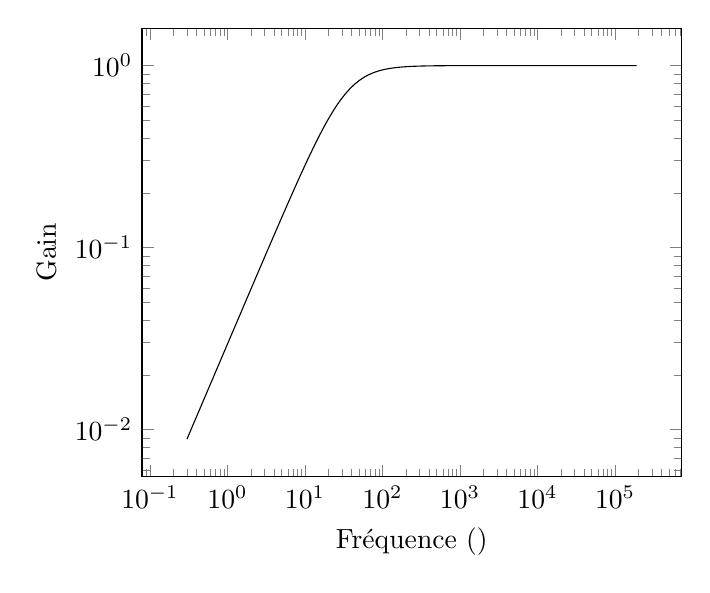
\begin{tikzpicture}
        \begin{loglogaxis}[
                xlabel={Fréquence (\hertz)},
                ylabel={Gain},
            ]
            \addplot[domain=0.3:1.9e5,samples=100]
            {1 / sqrt(1+1/(2*pi*10e3*470e-9*x)^2)};
        \end{loglogaxis}
    \end{tikzpicture}
    \qquad
    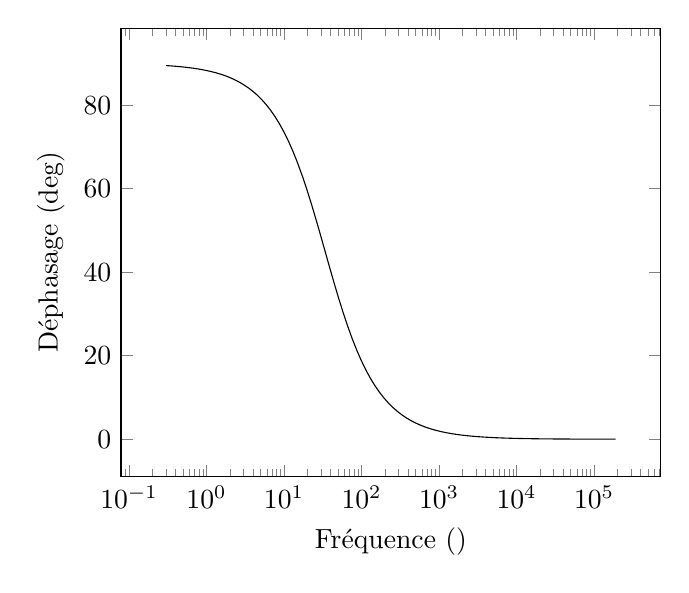
\begin{tikzpicture}
        \begin{semilogxaxis}[
                xlabel={Fréquence (\hertz)},
                ylabel={Déphasage (deg)},
            ]
            \addplot[domain=0.3:1.9e5,samples=100]
            {atan(1/(2*pi*10e3*470e-9*x)};
        \end{semilogxaxis}
    \end{tikzpicture}
    \caption{Courbes caractéristiques du filtre passe-haut}
    \label{fig:graphes-ph}
\end{figure}

\begin{figure}[h!]
    \centering
    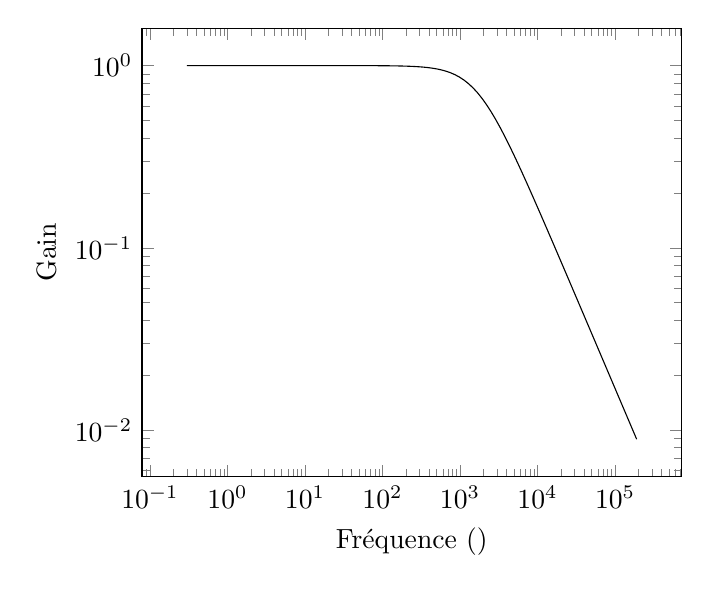
\begin{tikzpicture}
        \begin{loglogaxis}[
                xlabel={Fréquence (\hertz)},
                ylabel={Gain},
            ]
            \addplot[domain=0.3:1.9e5,samples=100]
            {1 / sqrt(1+(2*pi*200*470e-9*x)^2)};
        \end{loglogaxis}
    \end{tikzpicture}
    \qquad
    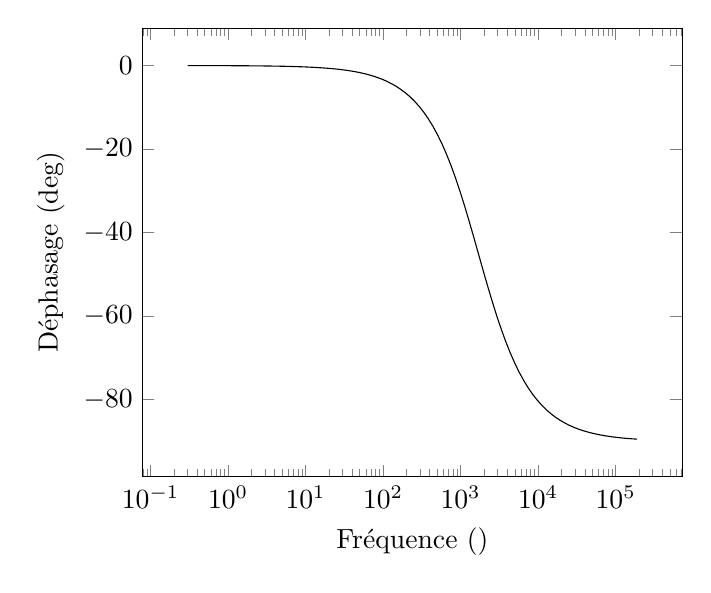
\begin{tikzpicture}
        \begin{semilogxaxis}[
                xlabel={Fréquence (\hertz)},
                ylabel={Déphasage (deg)},
            ]
            \addplot[domain=0.3:1.9e5,samples=100]
            {atan(-2*pi*200*470e-9*x)};
        \end{semilogxaxis}
    \end{tikzpicture}
    \caption{Courbes caractéristiques du filtre passe-bas}
    \label{fig:graphes-pb}
\end{figure}

Ces résultats sont illustrés par des graphes dans
les figures~\ref{fig:graphes-ph} et~\ref{fig:graphes-pb},
avec en abcisse la pulsation
et en ordonnée le gain et le déphasage.
Les tendances découvertes sont en pointillés.
Ici, les potentiomètre 2 est réglé à $20\,\%$ et le 3 à $100\,\%$,
donc $R_2 = 200\,\ohm$ et $R_3 = 2\,\kilo\ohm$.

Nous utilisons une échelle logarithmique pour les fréquences
ou pulsations, ainsi que pour les gains.
Les raisons de ce choix sont expliquées dans
la section~\ref{subsec:approx-lin/pres/loglog}.

Enfin, pour la combinaison des deux filtres,
les fonctions de transfert sont multipliées,
donc les gains sont multipliés et les déphasages sont additionnés.%
\footnote{
    Cela découle des propriétés du module et de l'argument.
    En effet, pour des complexes $x$ et $y$,
    on a $|xy| = |x||y|$ et $\arg(xy) = \arg x + \arg y$.
}
Le résultat est illustré dans la figure~\ref{fig:graphes-bande}.

\begin{figure}[h!]
    \centering
    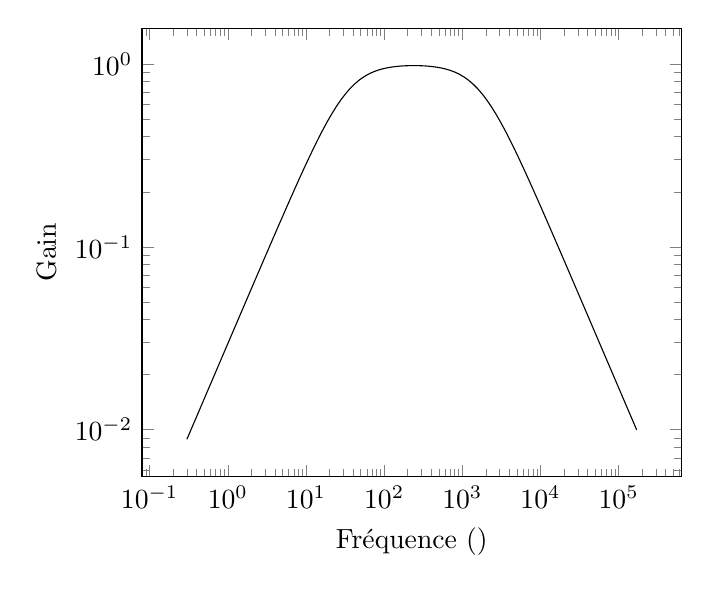
\begin{tikzpicture}
        \begin{loglogaxis}[
                xlabel={Fréquence (\hertz)},
                ylabel={Gain},
            ]
            \addplot[domain=0.3:1.7e5,samples=100]
            {1 / sqrt(1+1/(2*pi*10e3*470e-9*x)^2)
                / sqrt(1+(2*pi*200*470e-9*x)^2)};
        \end{loglogaxis}
    \end{tikzpicture}
    \qquad
    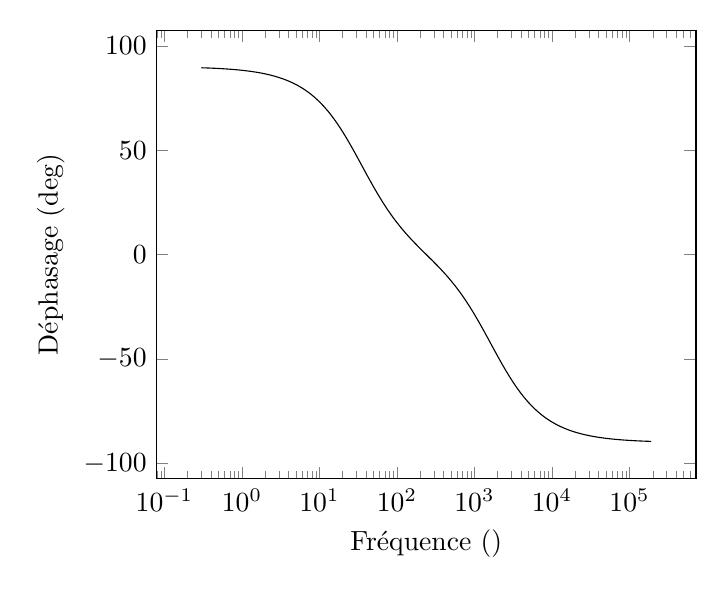
\begin{tikzpicture}
        \begin{semilogxaxis}[
                xlabel={Fréquence (\hertz)},
                ylabel={Déphasage (deg)},
            ]
            \addplot[domain=0.3:1.9e5,samples=100]
            {atan(1/(2*pi*10e3*470e-9*x))+atan(-2*pi*200*470e-9*x)};
        \end{semilogxaxis}
    \end{tikzpicture}
    \caption{Courbes caractéristiques de la combinaison des deux filtres}
    \label{fig:graphes-bande}
\end{figure}

Nous noterons les pulsations de coupure
$\omega\ind{bas} = 1/R_2C_2$ et $\omega\ind{haut}=1/R_3C_3$,%
\footnote{Nous omettrons les parenthèses lorsque cela améliore la lisibilité.}
appelées \emph{pulsations de coupure}.
Elles indiquent le passage d'un comportement à l'autre.
Nous expliquerons l'origine de ces valeurs en détail dans
l'annexe~\ref{chap:filtres-gen}.
